\chapter{membrane-equilibrium}

%\begin{introduction}
%	\item 红外光谱及其产生(理解)
%	\item 红外光谱仪及其结构(了解)
%	\item 红外光谱解谱(熟悉)
%	\item 拉曼光谱及其衍生(理解)
%\end{introduction}

\hypertarget{week4-1-membrane-equilibrium}{%
	\subsection{Week4-1 Membrane
		Equilibrium}\label{week4-1-membrane-equilibrium}}

\hypertarget{terms}{%
	\subsubsection{terms}\label{terms}}

\begin{itemize}
	\item
	extensive property: depend on the size or amount. follows additive rule.
	
	\begin{itemize}
		\item
		intensive property: e.g. density. 
	\end{itemize}
	\item
	for intensive properties, define partial molar quantity:
	\(\overline{Y_i}=\left(\frac{\partial Y}{\partial n_i}\right)_{T,P,n_j}\)
	
	\begin{itemize}
		\item
		then we can apply the additive rule.
	\end{itemize}
	\item
	chemical potential: PMQ of Gibbs free energy
	\begin{theorem*}{Definition of chemical potential}{}
		\[\mu_i=\mu_i^0+RT\ln a_i\]
	\end{theorem*}
	
\end{itemize}


\hypertarget{chemical-potential-equlibrium}{%
	\subsubsection{chemical potential
		equlibrium}\label{chemical-potential-equlibrium}}

\begin{itemize}
	\item
	for an open system (where \(n\) may vary but \(\mu\) doesn't vary
	under constant \(T,P\))
	\[\mathrm{d}G=\sum_i \mu_i\mathrm{d} n_i\]
	\item
	for a multiphase system \underline{in equilibrium}, which is separated
	by semi-permeable membrane
	
	\begin{itemize}
		\item
		for each component \(\mu_i\) should be the same and constant in all
		systems 
		\item
		only when this component is permeable. (\(\mathrm{d} n_i\neq 0\)) 
		\item
		when not in equilibrium, \(\mu\) may change first. But we only
		calculate about the equilibrium state 
	\end{itemize}
	
	\begin{figure}
		\centering
		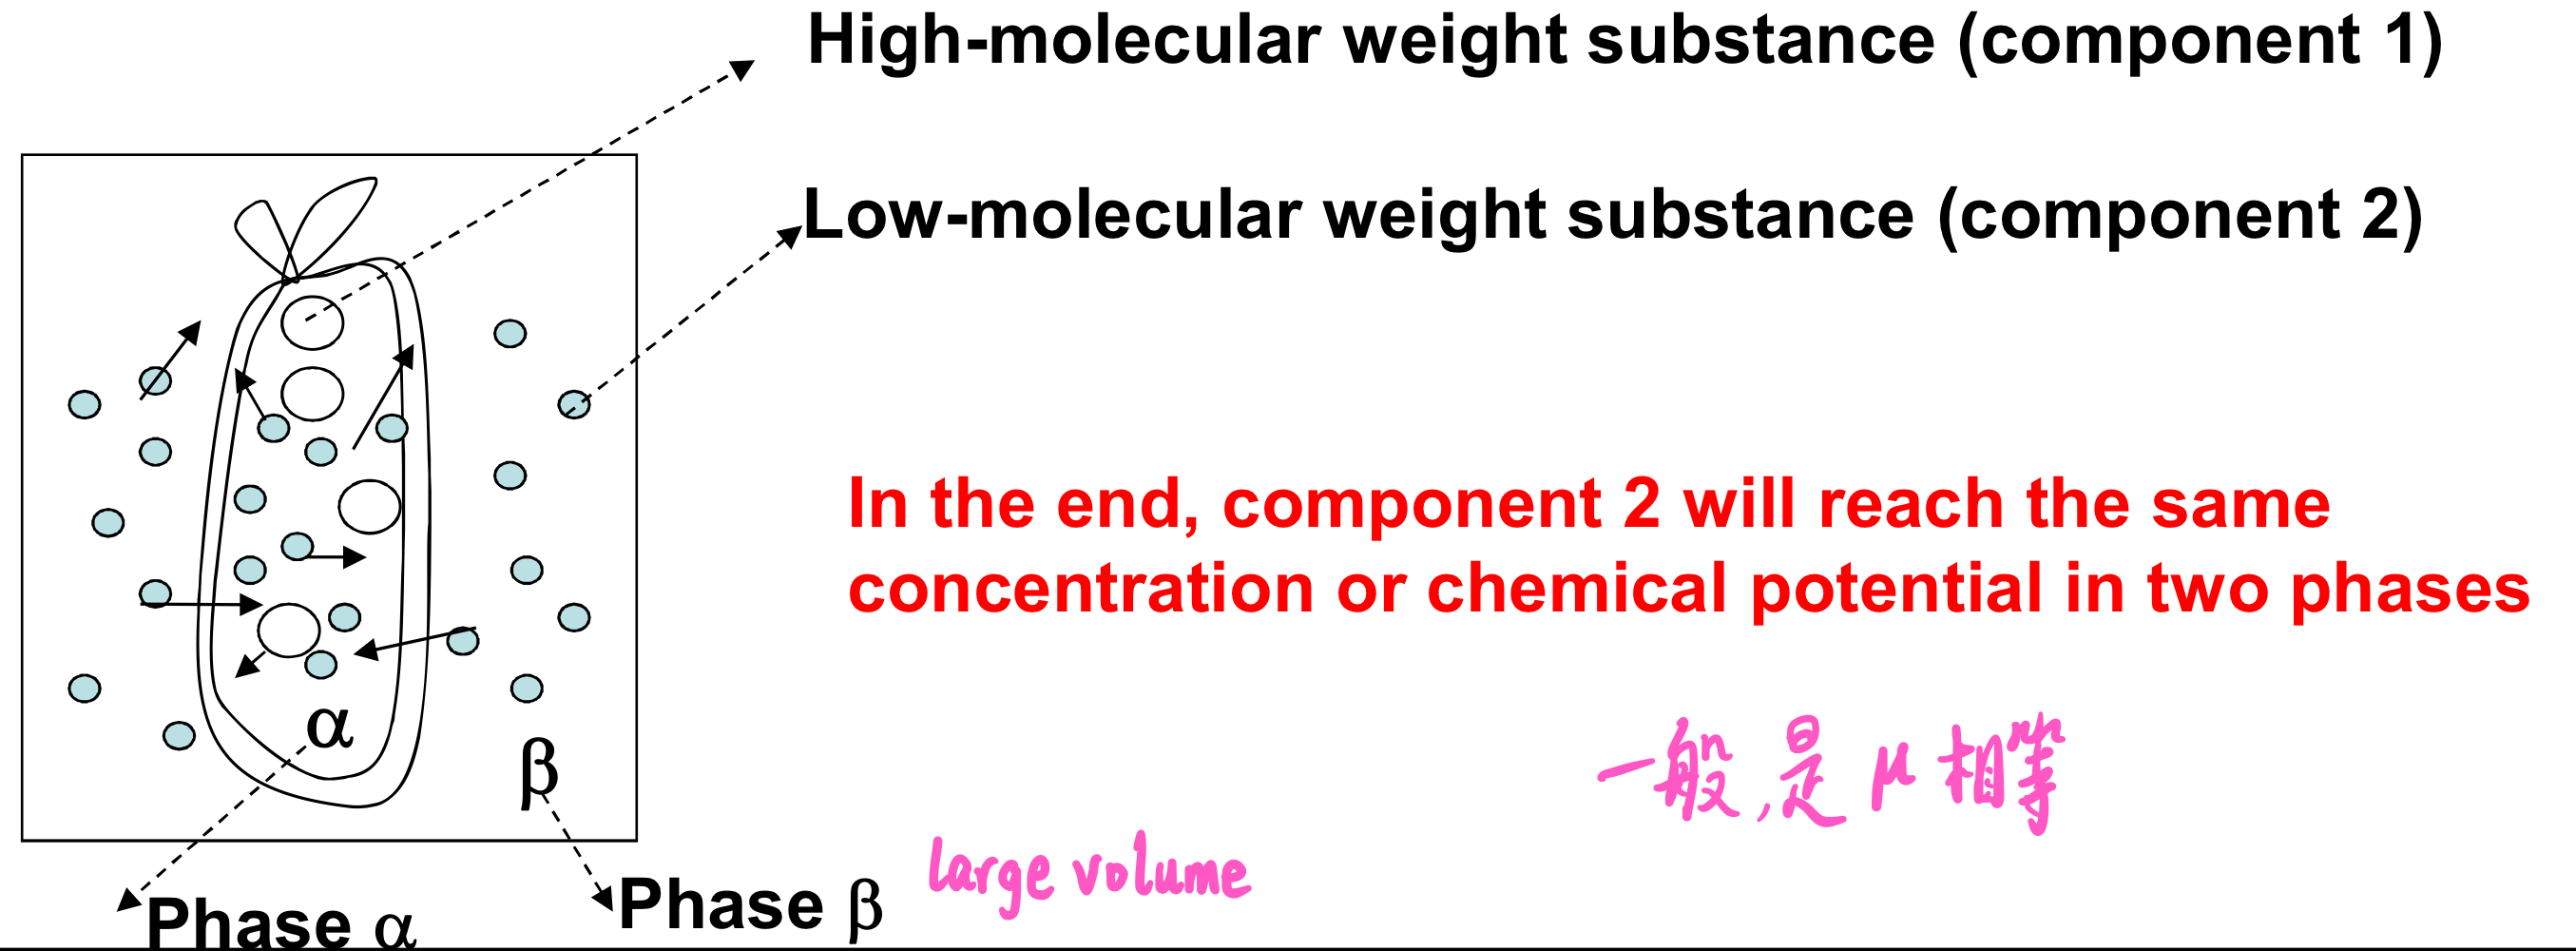
\includegraphics{E:/undergraduate_study/study/abroad study/2021 NUS/study/LSM3243/notes/4_1.png}
		\caption{}
	\end{figure}
	
	dialysis equilibrium
	\item
	when equlibrium is broken
	
	If only one side (\(\alpha\)) has solute A of molar concentration
	\(C\) that cannot pass through semi-permeable membrane. On the other
	side (\(\beta\)) is pure water with the same \(T\) and \(P\) (pressure
	of amtosphere on the liquid).
	
	\begin{figure}
		\centering
		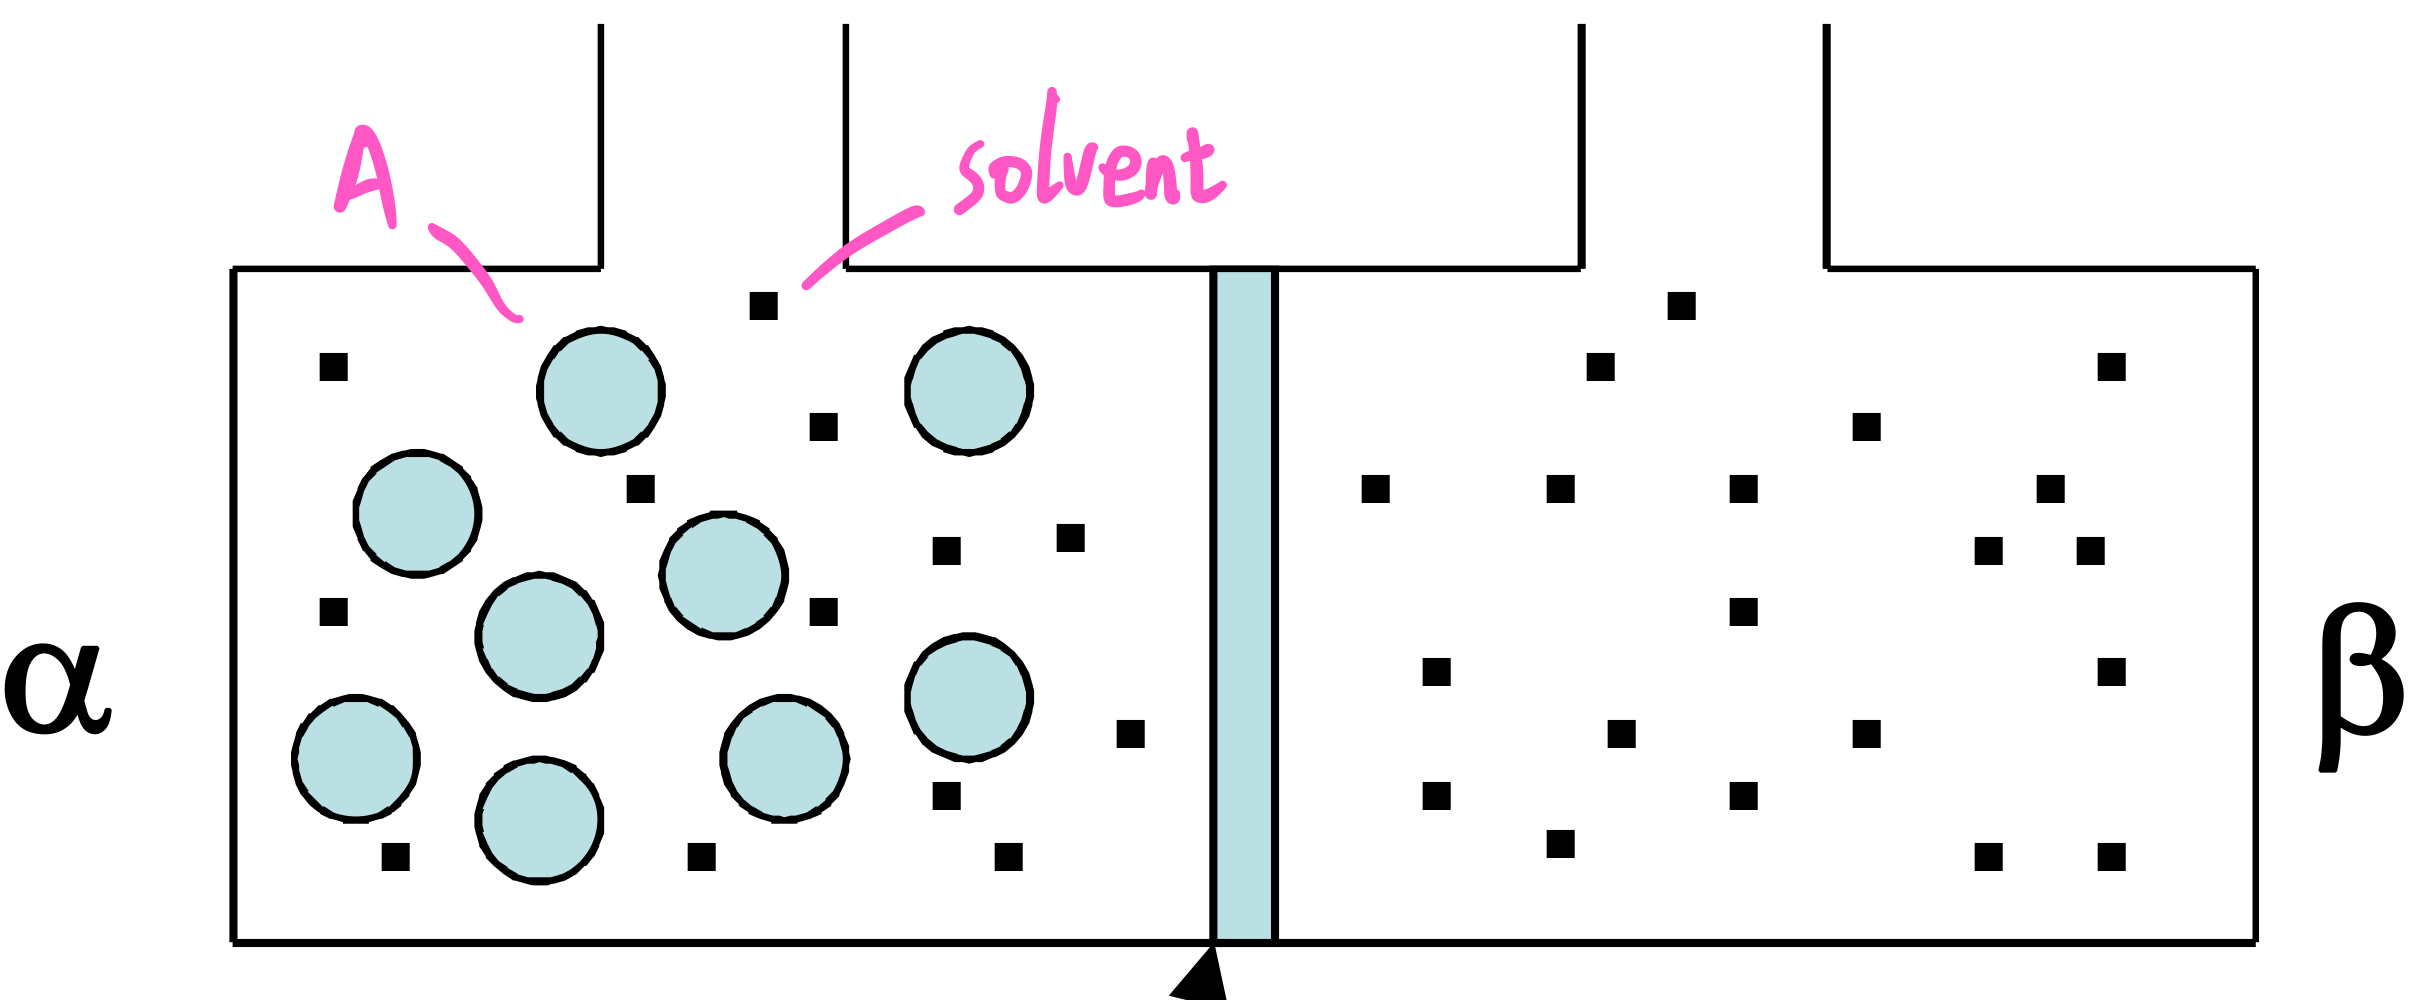
\includegraphics{E:/undergraduate_study/study/abroad study/2021 NUS/study/LSM3243/notes/4_2.png}
		\caption{4\_2}
	\end{figure}
	
	\begin{itemize}
		\item
		equilibrium can never be reached. \textbf{Osmotic pressure} is
		generated. 
		\item
		Imagine we change the pressure to achieve equlibrium, with
		approximation, we can get
		
		\[\pi=P^\alpha-P^\beta=RTC\]
		\item
		the solute can be either marcomolecules or small molecules
	\end{itemize}
\end{itemize}

\hypertarget{donnan-effect}{%
	\subsubsection{Donnan effect}\label{donnan-effect}}

the ion may start transfering, but have to keep electrical neutrality.

Donnan effect: when one side contains impermeable charged molecule,
concentrations of ions A,B in different side are different.

\begin{figure}
	\centering
	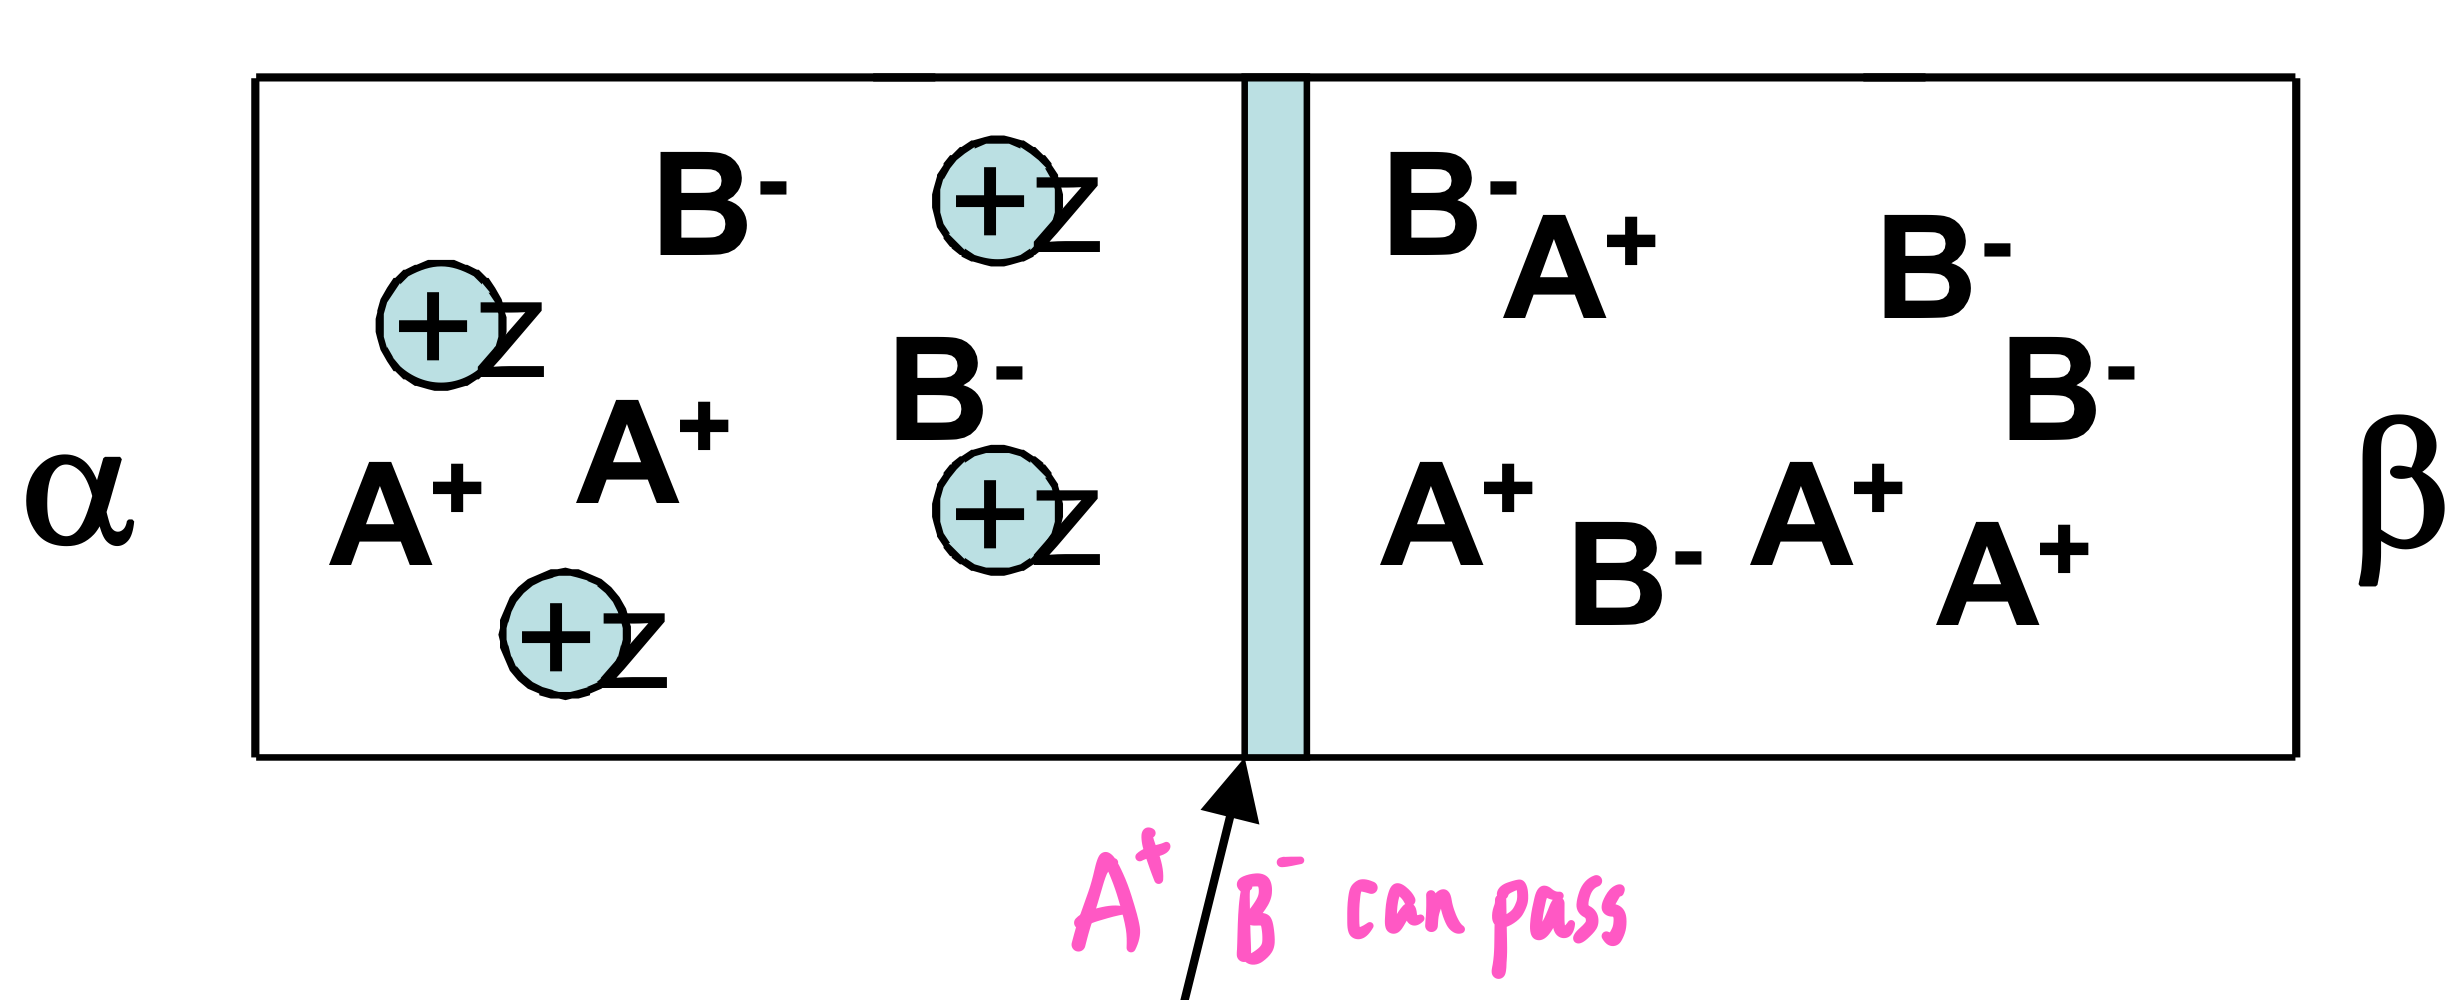
\includegraphics{E:/undergraduate_study/study/abroad study/2021 NUS/study/LSM3243/notes/4_3.png}
	\caption{4\_3}
\end{figure}

Write the chemical potential

\[\mu_1=\mu_{\ce{A}}^0+\mu_{\ce{B}}^0+RT\ln C_{\ce{A}}^\alpha+RT\ln C_{\ce{B}}^\alpha\\
\mu_2=\mu_{\ce{A}}^0+\mu_{\ce{B}}^0+RT\ln C_{\ce{A}}^\beta+RT\ln C_{\ce{B}}^\beta\\\]

At equlibrium, \(\mu_1=\mu_2\)

\[C^\alpha_{A}\cdot C^\alpha_{B}=C^\beta_{A}\cdot C^\beta_{B}\]

Note \(z\) is the charge and \(C_M\) is concentration of the
marcomolecule. According to electrical neutrality, let

\[C^\alpha_{A}+zC_M=C^\alpha_{B}=a\\
C^\beta_{A}= C^\beta_{B}=b\\
r=\dfrac{zC_M}{2C^\beta_{A}}\]

then solve it

\[r_D=\dfrac{C^\beta_{A}}{C^\alpha_{A}}=\dfrac{C^\alpha_{B}}{C^\beta_{B}}=r+\left(r^2+1\right)^{0.5}\]

If A is \(\ce{H+}\), then
\(\mathrm{pH}^\alpha-\mathrm{pH}^\beta=\log r_D\)

\hypertarget{combined-effect-membrane-potential}{%
	\subsubsection{combined effect: membrane
		potential}\label{combined-effect-membrane-potential}}

Consider this situation. \(\ce{Na+}\) won't pass through because of the
electric potential. Chemical potential equilibrium can never be reached,
as in the example about osmotic pressure. This system looks like
\underline{the cell} where no ions can freely pass through.

\begin{figure}
	\centering
	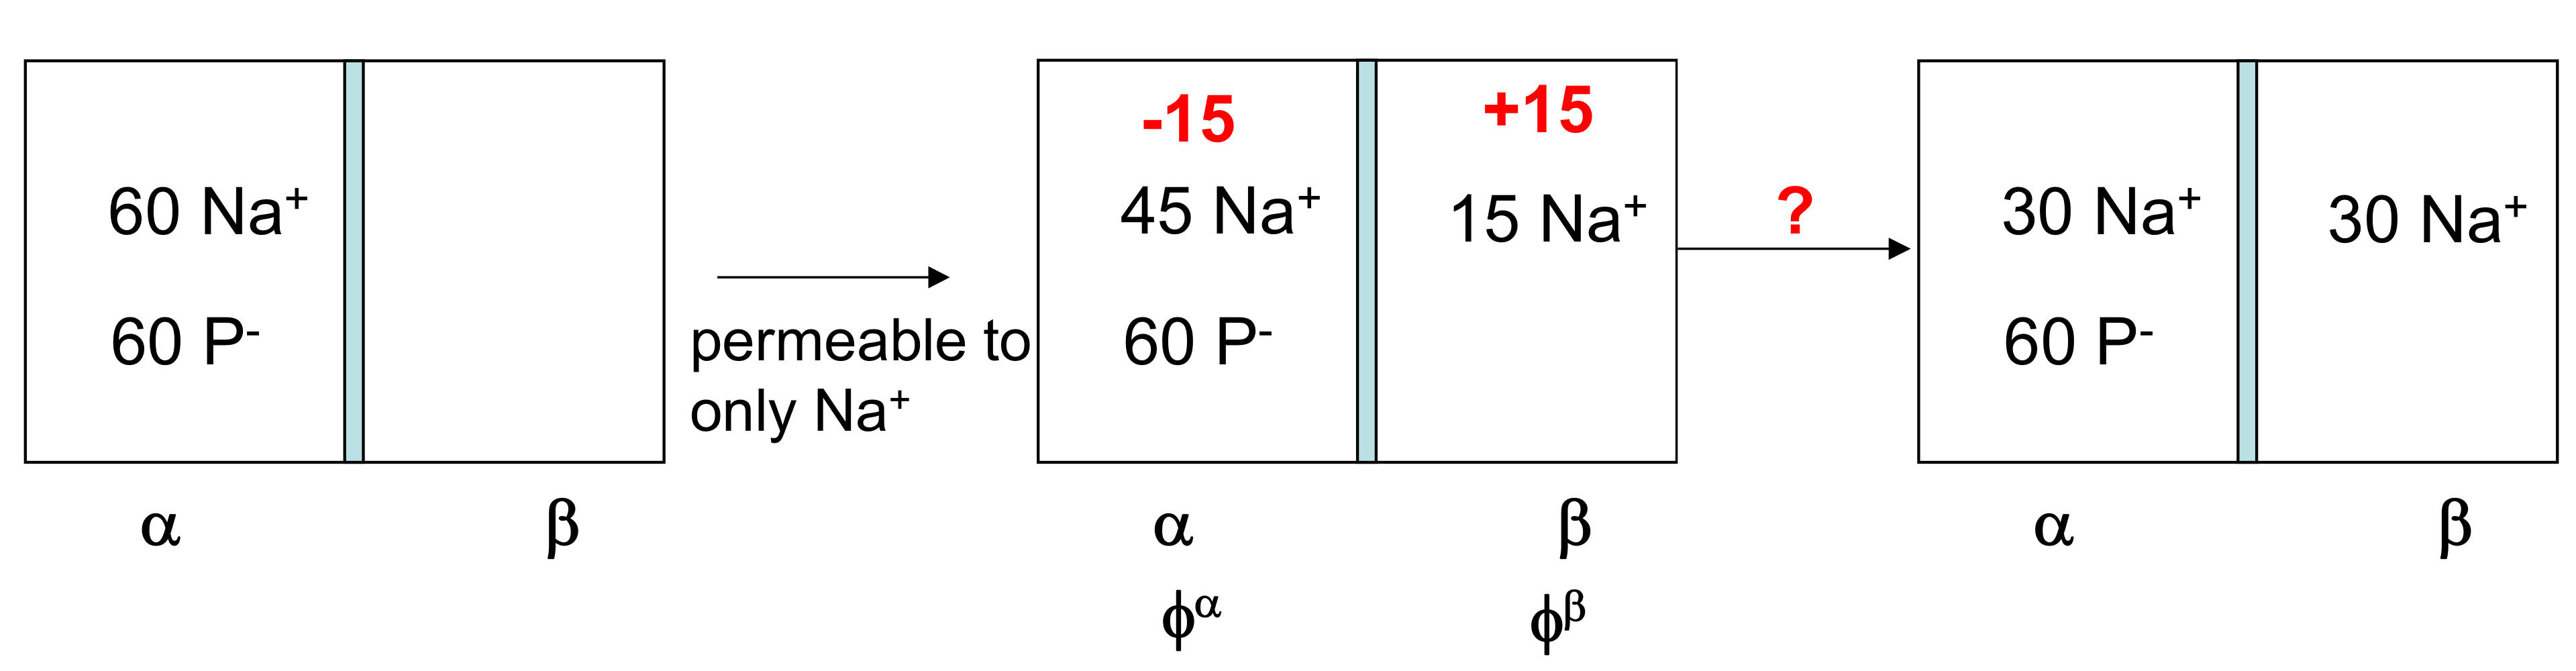
\includegraphics{E:/undergraduate_study/study/abroad study/2021 NUS/study/LSM3243/notes/4_4.png}
	\caption{}
\end{figure}

Part two of this section refers to the effect of different
concentration, while part three refers to the effect of charged
molecules.

Define electrochemical potential as their combination

\[\mu^\prime=\mu+Zf\phi\]

where \(Z\) is charge, \(f\) is Faraday constant, \(\phi\) is the
relative electric potential.

At equlibrium, for single ion A on one side:

\[\Delta\varphi=\varphi^{in}-\varphi^{out}=-\dfrac{RT}{Zf}\ln\dfrac{c^{in}}{c^{out}}\]

Ionic concentration difference and membrane potential are generated
simultanously. Maintaining a concentration difference, we get membrane
potential. Still, those which cannot pass through the membrane don't
contribute.

For multiple ions:

\[\Delta\varphi=\varphi^{in}-\varphi^{out}=-\dfrac{RT}{Zf}\ln\dfrac{\sum\limits_{positive} p_ic_{i}^{in}+\sum\limits_{negative} p_jc_{j}^{out}}{\sum\limits_{positive} p_ic_{i}^{out}+\sum\limits_{negative} p_jc_{j}^{in}}\]

where \(p_i\) is permeability. The cell mainly regulates permeability
and sometimes concentration.

\begin{quote}
	summary:
	
	By putting charged marcomolecules and selectively letting ions pass
	through, the cell sets up the difference of concentration of ions as
	well as the electrical potential, acting as the fundation of activities
	like neural signaling.
\end{quote}

\hypertarget{in-addition}{%
	\subsubsection{in addition}\label{in-addition}}

inference of osmotic pressure

\[\mu_1^\alpha=\mu_1^0(T,P^\alpha)+RT\ln c_1^\alpha y_1^\alpha\\
\mu_2^\beta=\mu_2^0(T,P^\beta)+RT\ln c_2^\beta y_2^\beta\]

where \(c\) is the molar concentration of water. Here it's approximately
the molar ratio (?)

Due to \(G=U+PV-TS\), \(\mu=V_0P\), \(V_0\) is molar volume of water.

When equilibrium, \(\mu_1^\alpha=\mu_2^\beta\). Assume \(y=1\) So

\[\mu_1^0(T,P^\alpha)-\mu_2^0(T,P^\beta)=V_0(P^\alpha-P^\beta)=-RT\ln\dfrac{c_1^\alpha}{c_2^\beta}\]
